%File: formatting-instruction.tex
\documentclass[letterpaper]{article}
\usepackage{aaai}
\usepackage{times}
\usepackage{helvet}
\usepackage{courier}
\usepackage{graphicx}
%Hans
\usepackage{subfigure}

\frenchspacing
\setlength{\pdfpagewidth}{8.5in}
\setlength{\pdfpageheight}{11in}
\pdfinfo{
/Title (Insert Your Title Here)
/Author (Put All Your Authors Here, Separated by Commas)}
\setcounter{secnumdepth}{0}  

% The file aaai.sty is the style file for AAAI Press 
% proceedings, working notes, and technical reports.
%
\begin{document}
\title{Efficiently Retrieving Images that We Perceived as Similar}
%\author{Hui-Ju Katherine Chiang$^{1}$, Shih-Han Wang$^{2}$, Jane Yung-jen Hsu$^{2}$\\
%$^{1}$Graduate Institute of Electronics Engineering, National Taiwan University, Taipei 10617, Taiwan\\
%$^{2}$Graduate Institute of Networking and Multimedia, National Taiwan University, Taipei 10617, Taiwan\\
%\{d01943033, r02944022\}@ntu.edu.tw, yjhsu@cise.ntu.edu.tw
%}
\maketitle
\begin{abstract}
\begin{quote}
Despite growing interest in using sparse coding based methods for image classification and retrieval, progress in this direction has been limited by the high computational cost for generating each image's sparse representation. To overcome this problem, we leverage sparsity-based dictionary learning and hash-based feature selection to build a novel unsupervised way to efficiently pick out a query image's most important high-level features that can determine to which group we would visually perceived as similar. The preliminary results based on L1 feature map show the method's efficiency and high accuracy from the visual cognitive perspective. Finally, we consider a more general problem of how to make the pre-learned dictionary to adaptively refine the features contained according to past queries.
%We propose a novel way to search natural images by higher-level features from the observations in human primary visual cortex to combine the simulation result of v1 neurons and expect to do large images search as a new cognitive architecture. We leverage sparsity-based dictionary learning and hash-based auto-learned feature selection algorithm to show fast images retrieval results. Finally, we consider a more general problem of how a learned dictionary might be related to large-scale data retrieval and expect to draw more attention to this important research.
\end{quote}
\end{abstract}

\section{Motivation and Introduction}
As the amount of digital data grows in unprecedented speed, new opportunities come with new challenges. The real value of big data lies in the ability to extract from it meaningful, even insightful information, rather than the ``big'' itself. Furthermore, many applications also require information to be retrieved \emph{fast}.
\emph{Efficient} similar image retrieval thus becomes an important problem in the field of artificial intelligence with many real-world applications. 
The task is closely related to the nature of \emph{human cognition} since any definition of \emph{similarity} is meaningful only when it coincides with human feeling. Though the similar-or-not decision comes intuitively in no time for human, to find a well-defined decision guideline for computers is extremely hard. To resolve this stark discrepency that can inhibit human-machine cooperation, in this paper, we propose a novel 
method %(need better wording instead of 'method')
that emulates several important aspects of actual neurophysiological mechanisms, including \emph{sparse coding} in primary visual cortex (V1), \emph{synaptic plasticity}, and \emph{mutual inhibition} between neurons. The mechanisms are not chosen randomly, instead, they complement each other's weak points for overall improvements without sacrificing efficiency.

Given unlabeled data, \emph{sparse coding} provides a class of algorithms capable of extracting higher-level features that are actually more cognitively effective than hand-picked ones by emulating partial activity of neurons. The features can be regarded as the most representative building blocks by which the input data can be reconstructed most \emph{efficiently} -- highest accuracy with fewest elements used. The features form the \emph{overcomplete} bases that resemble the \emph{receptive fields} of neurons of in the visual cortex, making sparse coding a more appropriate medium than other widely-used computer vision features such as SIFT (Lowe 1999), GIST (Oliva et al. 2001), HOG (Dalal et al. 2005) etc., to bridge human cognition and algorithmic way of learning.

Unfortunately, though there are works (Ge et al. 2013) that tackle the image search problem by first representing query images as their sparse codes, the high computational cost involved in sparse code calculation renders it infeasible for (near) realtime retrieval tasks. Thus, we proposed in this paper a novel approach to overcome the performance bottleneck by a change of perspective: equipped with already-learned features stored as a \emph{dictionary}, can we filter out the dominant features \emph{directly} from an image, without resorting to the \emph{complete} set of its sparse code? By regarding those selected features collectively as the image's \emph{hash value}, the method actually transforms the sparse coding based approach to one more similar to efficient hash-based methods. In the following, we would use basis and feature interchangeably, and refer to the group of importatnt features learned as the \emph{dictionary}.

Considering the fact that sparse representation is based on an \emph{overcomplete} basis (Olshausen and Field 1996), we use concepts similar to that of inner-products and orthogonal decompositions to aid our feature selection. Overcomplete basis emerges as a natural result of the \emph{sparsity} constraint. Sparsity requirement goes against using only independent basis to assemble other important features, instead, if a feature is popular and representative enough, it would be more beneficial to add it into the dictionary to improve sparsity. As a result, apart from the robustness it provides, the seemingly redundant overcompleteness implies the vectors' independent importance in representing different types of data. This forms the reason behind choosing similar features only exclusively, i.e. similar features are mutually inhibitive. 

By combining the inhibition-like decomposition scheme with an additional mechanism that emulates synaptic plasticity, we are able to come up with a retrieval system with hash-based-like efficiency, and performance comparable to GIST-based approach. Experiments based on \emph{SUN397 scene benchmark} confirmed the effectiveness and efficiency of our method.

%Some people have images search problem with the representation of sparse codes proposed by (Ge et al. 2013). However, finding sparse codes has high computational costs on doing effective real time search. We propose a novel approach to solve this problem by using overcomplete basis in dictionary rather than computing sparse codes and we will show that our approach is effective in natural image. 

%There are many researches studying about how to make image retrieval effective. Conventionally, there are three steps in large-scale content-based image retrieval when given a set of indexed images and a query image. The first is feature extraction. Many complex approaches are developed to find effective image representation to encode a variety of images. Secondly, dimension reduction is important to speed up the retrieval process. Finally, effective metric is needed to compute the similarity between features. Compared to the traditional framework we propose a different solution without the part of feature extraction to solve this problem by the plausible model of visual cortex—sparse coding.

%Sparse representation based on an \emph{overcomplete} basis (Olshausen and Field 1996), inspired by mammalian striate cortex mechanism from neural science community has been widely applied in many computer science fields, such as data compression, speech recognition and image denoising,  etc. (Sivaram 2010), (Wright et al. 2009).  One important property of sparse coding is that it can extract from data higher-level features that are actually more cognitively effective than hand-picked ones by simulating partial activity of neurons.  
%According to promising neural science theory and the high performance of algorithms developed within decades, we assume that sparse coding which simulates mammalian visual cortex activities is a very efficient approach to find the latent features compared to traditional unsupervised learning such as PCA. We also assume that neuron simulation-based approach for image representation is better than other widely used computer vision features including SIFT (Lowe 1999), GIST (Oliva et al. 2001), HOG (Dalal et al. 2005) and etc. because we have our visual system as promising evidence to support. 

\section{Proposed Retrieval System}

\subsection{System framework}
\label{subsec:framework}

\begin{figure}[!h]
		\centering
		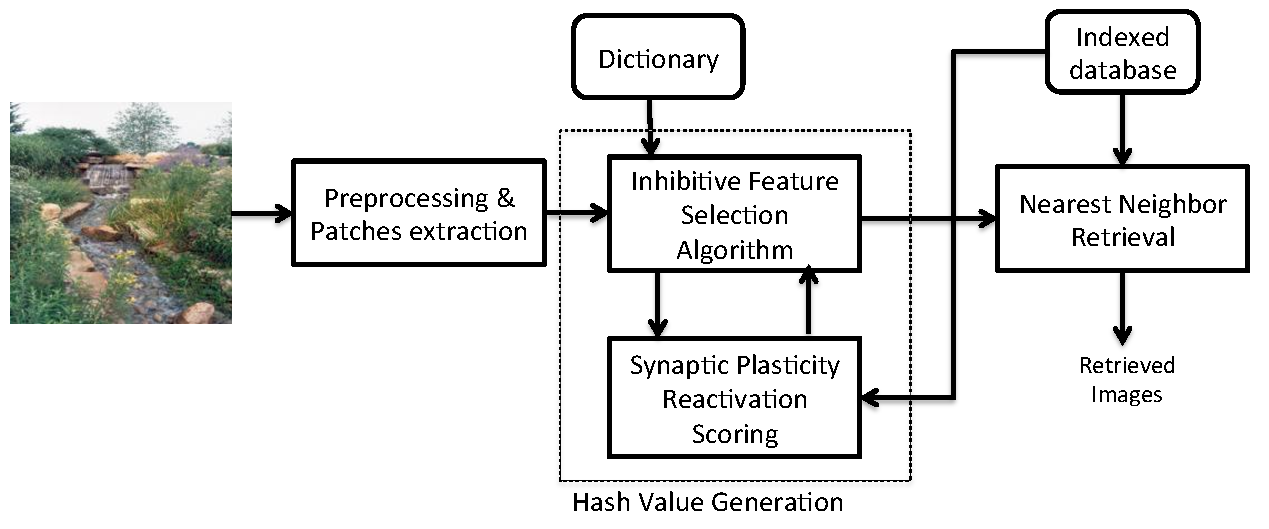
\includegraphics[width=3.0in]{figures_dir/aaai_systemDiagram.pdf}
		\caption{Proposed system.}
		\label{fig:framework}
\end{figure}

\subsection{Image Preprocessing}
Before feeding into the system, all images including those used for dictionary training are first whitened. Whitening makes the input less redundant by removing the correlations between neighboring pixels. This step is very fast while allowing significant improvement in feature learning quality, as the features to be learned would become less correlated and of the same variance. Since the sparse coding algorithm is based on.... the learned features 
 
%Given a query natural image, we firstly decorrelate the image to equalize the variance which is also employed in preprocessing for dictionary due to potential factual and corrupted and this also roughly simulate spatial-frequency reponse characteristic of retinal ganglion cells proposed by (Olshausen 1997) in our cognitive system.  We then uniformly select several image patches to extract a certain pattern of the image. We feed all extracted vectors into our auto-learned feature selection algorithms to encode the data. Finally, we use L2 distance as default metric to compute similarity score. The system diagram is shown in Fig.~\ref{fig:framework}.

\subsection{Offline Unsupervised Dictionary Learning}
\label{subsec:dictionary}
Sparse-based dictionary learning has been proved to be especially effective in capturing discriminative features of scene images. We use the \emph{Efficient sparse coding algorithms} proposed in (Lee et al. 2007) to build the dictionary of features from a learning set of 1000 images of size $200\times200$ pixels.
%Given unlabeled scene images, the effective sparse coding proposed by (Lee et al. 2007) captures succinct feature with higher meanings and generate a dictionary with overcomplete bases which are effective to represent the image in data set given the corresponding sparse code. The basic descriptions such as edges and line segments are efficiently encoded into atoms of dictionary so we will pre-trained the dictionary as our dimension reduction projection bases.
\begin{figure}[!ht]
		\centering
		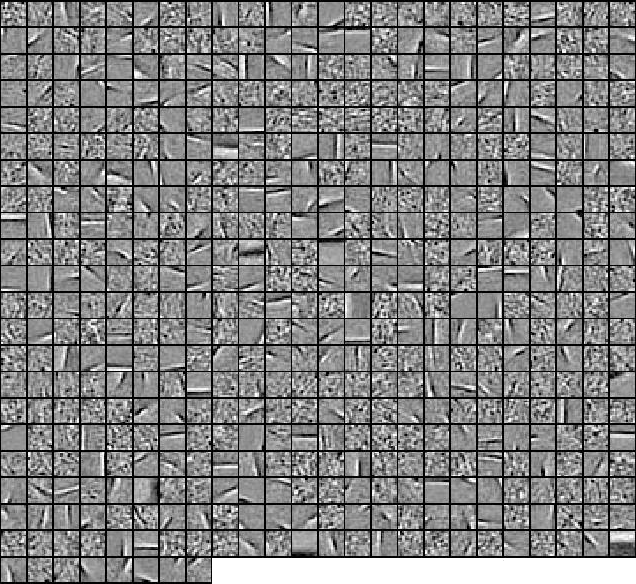
\includegraphics[width=2.2in]{figures_dir/dict.png}
		\caption{The Learned Dictionary}
		\label{dictionary}
\end{figure}
\subsection{Hash Value Generation}
\subsubsection{Inhibitive Feature Selection Algorithm}
-Sparcity: since a vector that best captures one feature is not necessarily independent from vectors that best capture other features

-Robustness vs entropy: when two elements are selected together with high probability, one of them becomes redundant as it provides merely any extra information. But this should not be the case.
Since our retrieval framework encode the image pattern of natural images into sparsity-based dictionary, we are motivated to select effective feature, especially those have high response to patches of natural images. Inspired by localitive sensitive hashing proposed by (Andoni et al. 2008), where high dimensional data can be projected to lower dimensional space with similarity preserving promise, we propose our novel algorithm to find out the atom of feature pattern in the dictionary to perform our hash-based dimensional reduction.

Firstly, we project our patches vector onto the atom of dictionary to get the highest values of the result for each vector of patches and have another zero array with the same size. We call those atoms strong responsive to the corresponding patches vector. Then, we set the value of each patches vector at corresponding atom of dictionary to be one.

Secondly, we substract the strong responsive atom from the corresponding patches vector in order to select second strong responsive atom with respect to the corresponding patches vector.

Iteratively, we will rank out the top n strong responsive atoms as our output for each patch vector. By this way, we can encode the raw data directly by the ranking of the response of corresponding atom based on sparsity based dictionary and we will show that the result has some effects consistent with our visual system.
\begin{figure}[!ht]
		\centering
		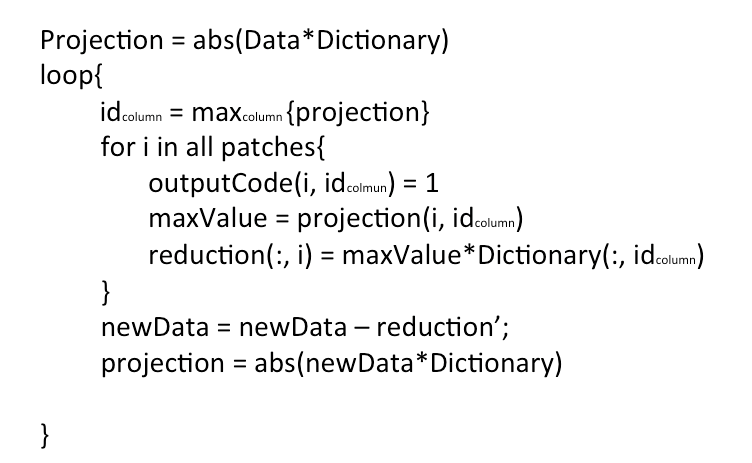
\includegraphics[width=.4\textwidth]{figures_dir/temp_algorithm1.png}
		\caption{Auto-learned feature selection algorithm (ALFSA)}
		\label{TEMP!!! Inhibitive Feature Selection Algorithm}
\end{figure}

\subsubsection{Synaptic Plasticity Reactivation Scoring}
%{Response Reactivation Scoring}
\begin{figure}[!ht]
		\centering
		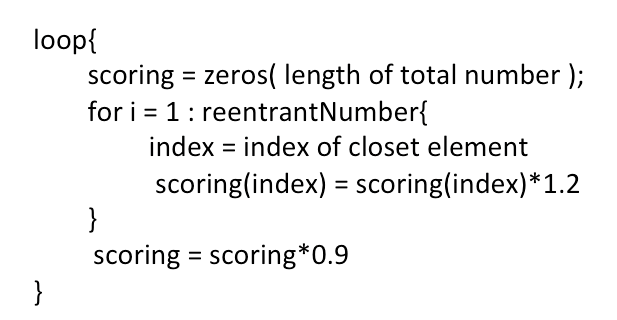
\includegraphics[width=.4\textwidth]{figures_dir/temp_algorithm2.png}
		\caption{Response Reactivation Scoring}
		\label{cottage_garden_top10_comparison}
\end{figure}
%%%%%%%%%%%%%%%%%%%%%%%%%%%%%%%%%%%%%%%%%
\begin{figure*}[!ht]
\centering
\subfigure{
   		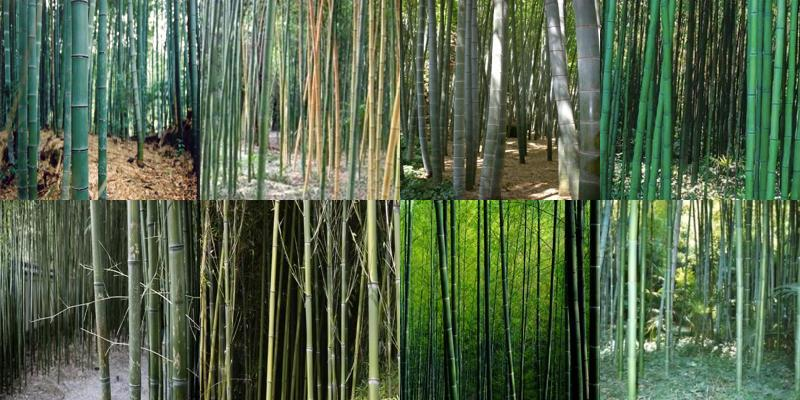
\includegraphics[width=2.3in]{figures_dir/bamboo_forest.jpg}	
        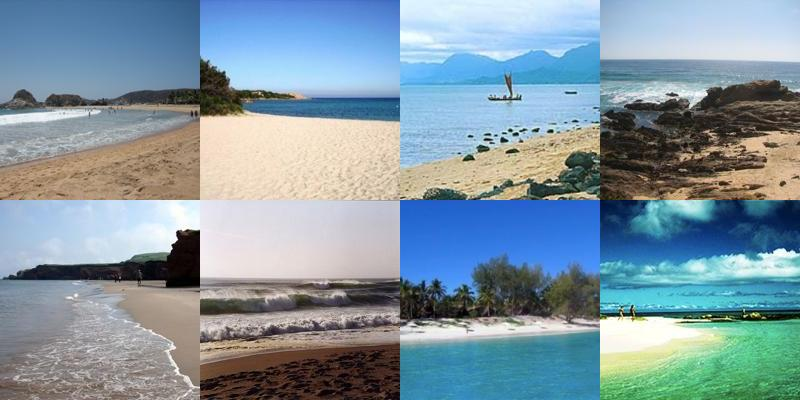
\includegraphics[width=2.3in]{figures_dir/beach.jpg}
		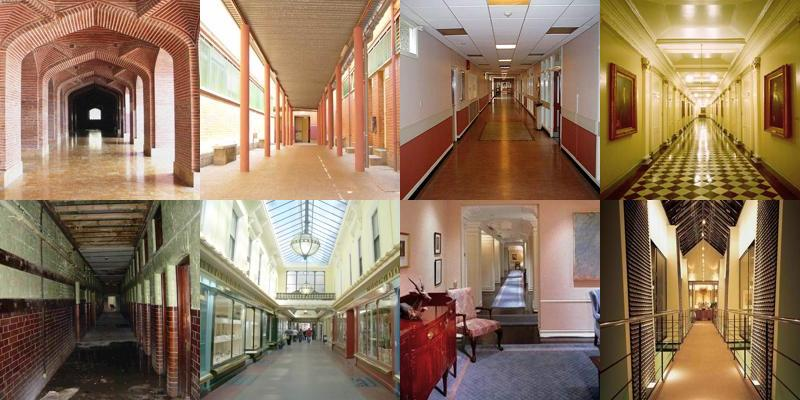
\includegraphics[width=2.3in]{figures_dir/corridor.jpg}
   \label{fig:subfig1}
 }

 \subfigure[Subfigure 2 caption][]{
   		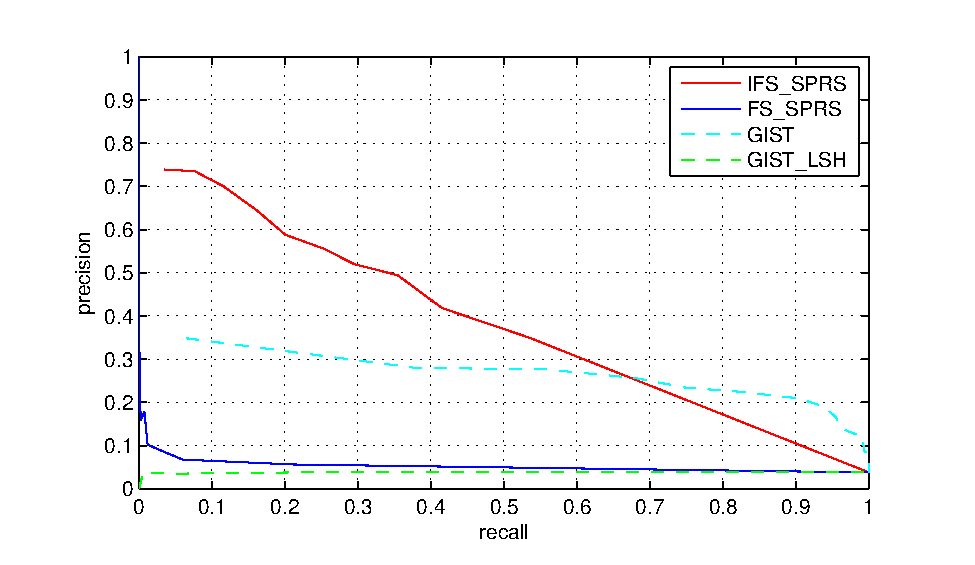
\includegraphics[width=2.33in]{figures_dir/bamboo_forest_10queries_4comparison_75.eps}   		
        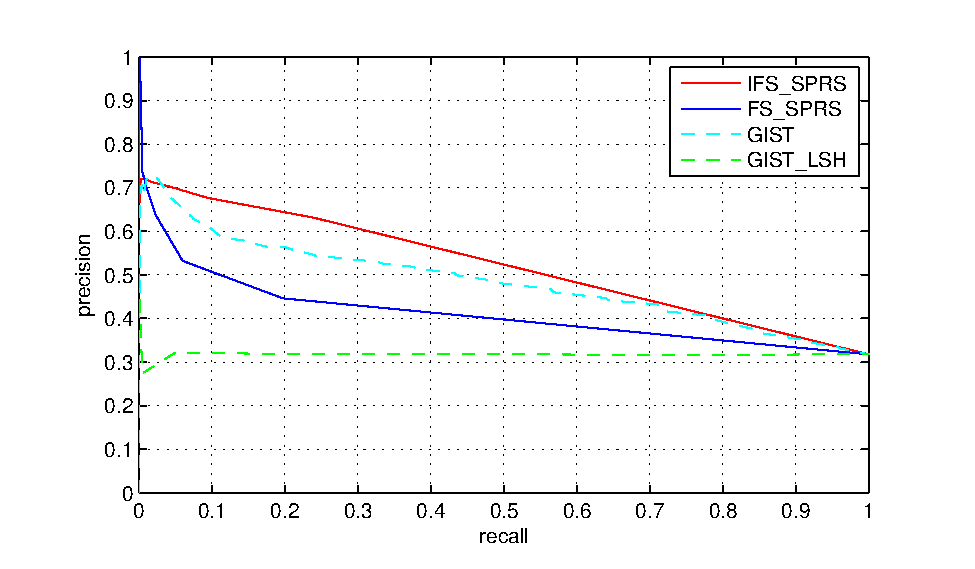
\includegraphics[width=2.33in]{figures_dir/beach_10queries_4comparison_75.eps}
        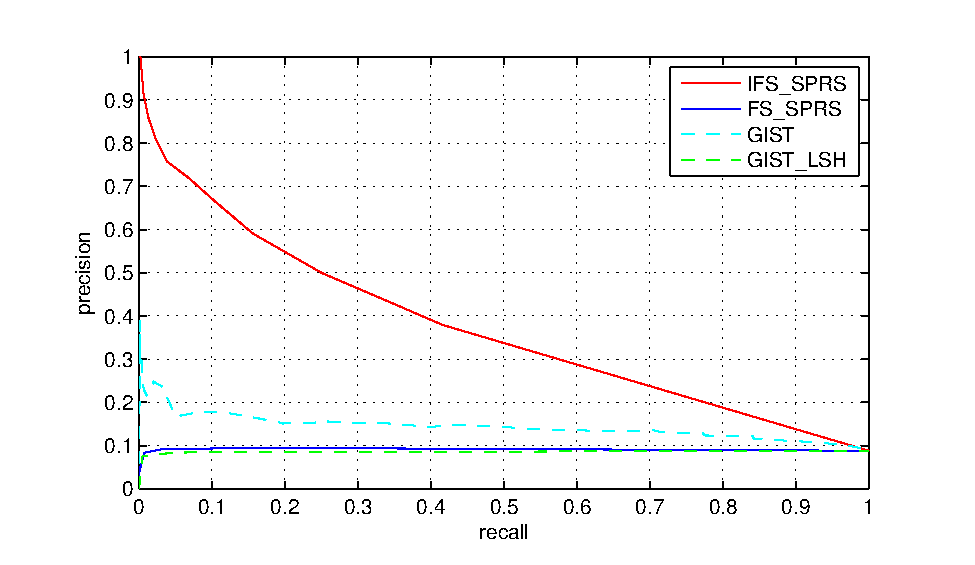
\includegraphics[width=2.33in]{figures_dir/corridor_10queries_4comparison_75.eps}
   \label{fig:subfig2}
 }

\label{for subfig}
\caption{Global figure caption}
\end{figure*}

\section{Experimental results}
We evaluate our proposed system on a subset of SUN397 database. Our database contains 10 categories from all three top-level partitions (indoor, outdoor natural, outdoor man-made): bamboo forest, beach, botanical garden, corridor, cottage garden, hayfield, mountain snowy, waterfallBlock, wheat field, and wine cellearBarrelStorage.  To accelerate training as well as later query stage, rather than directly representing the whole image by human-tuned feature sets, we randomly extract !!! $14\times14$ pixels patches from each images.
%We evaluate our proposed system on a subset of scene images which is a version of MIT SUN dataset, SUN397 scene benchmark, from (!!!).  Our subdataset consist of 3,583 scene images that have been grouped into 10 different classes: bamboo\_forest, beach, botanical\_garden, corridor, cottage\_garden, hayfield, mountain\_snowy, waterfallBlock, wheat\_field, wine\_cellearBarrelStorage. Original images in the dataset have different sizes so we resize them into the size of 200x200 pixels. Rather than represent them with the state of the art manual-turned feature, we extract small 14x14 pixels image patches directly by uniform random selection. We call our auto-learned feature selection method ALFS and we will evaluate our method in two parts, the improvement, from naive method to our design alogrithm showing the progress,under our sparsity dictionary and the comparison with the well known human-turned global feature, GIST.

%\begin{figure}[!ht]
%		\centering
%		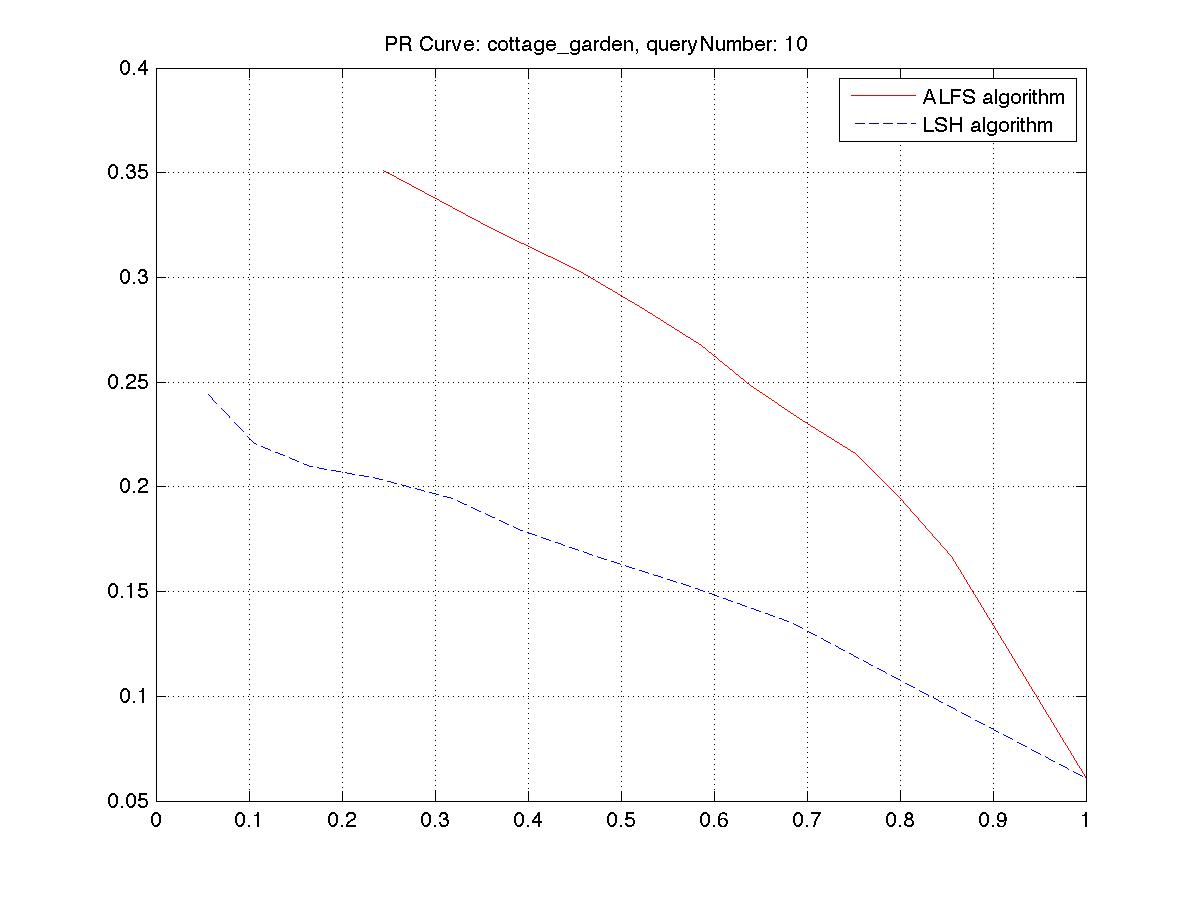
\includegraphics[width=.4\textwidth]{figures_dir/cottage_garden_top10_comparison.jpg}		
%		\caption{Precision and recall curve}
%		\label{cottage_garden_top10_comparison}
%\end{figure}

\subsection{Improvement under sparsity dictioanry framework}
Under our sparsity dictioanry framework inspired from neuron activity, we implemented two encoding method: one is our novel ALFS algorithm, which is called Neuron\_ALFS in figures. Another one is inspired from localitive sensitive hashing method, projecting the raw images patches onto the learned dictionary, which is our first method to explore the effectiveness of image retrieval under such a novel sparsity dictionary framework. Although LSH-based method requires Gaussian random distribution, it also works fair to be discriminative  under our sparse coding framework by simple hash projection on learned dictionary. While we apply this method on our learned basis vector with normal distribution, certain latent similar feature seems to be preserved after the projection to retrieve similar images.
We call this naive idea inspired from traditional LSH as Neuron\_LSH in figures.

\subsection{Comparison with Human-tuned feature methods}
Due to our scene dataset, to be fair, we employ GIST features to do the evaluation. For comparison, we extract GIST features proposed by (!!!) directly from 200x200 pixels images 
Due to the most state of the art working under different framework from us,  we compare our ALFS method with LSH-based scheme under our spetial sparse coding framework as the baseline and we will show how much we have improved under this novel framework for image retrieval as an example. 


%%%%%%%%%%%%%%%%%%%%%%%%%%%%%%%%%%%%%%%%%
%%%%% Random 100 queries PR-curve
%%%%%%%%%%%%%%%%%%%%%%%%%%%%%%%%%%%%%%%%%
\begin{figure}[ht]
	\centering
	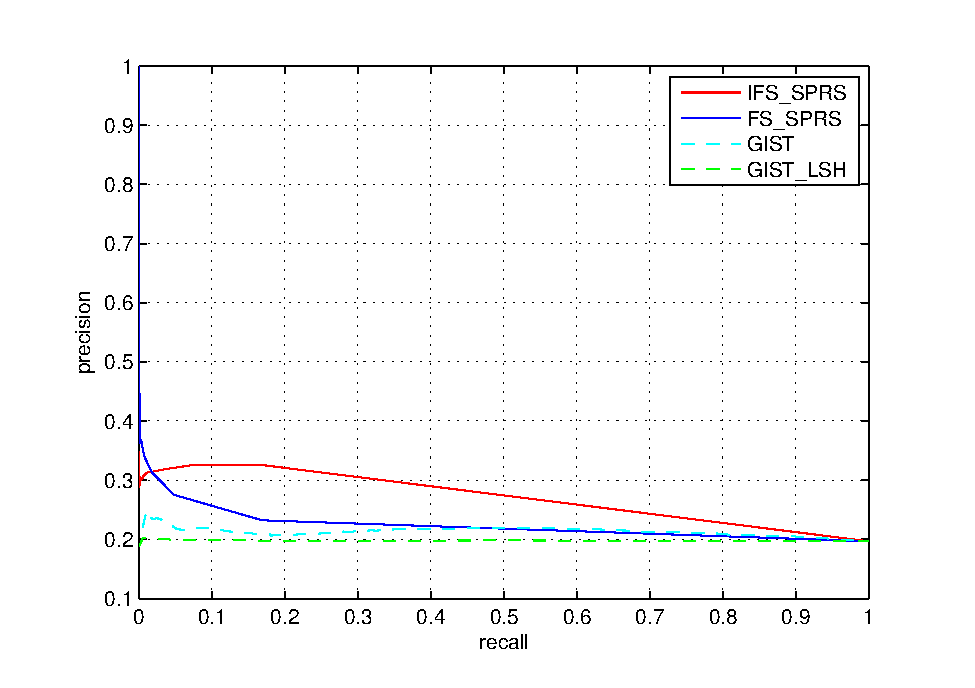
\includegraphics[width=3.5in]{figures_dir/round4_random100_4comparison_75.eps}
	\caption{hello}
	\label{random 100 queries}
	
\end{figure}




\section{Conclusion}
Rather than traditional human-turned feature extraction our cognitive system based on sparse coding successfully combine proposed novel auto-learned feature selection algorithm with sparsity-based dictionary to create ouw own discriminative code to retrieve natural images with high performance. The sparsity-based dictionary which capture basic elements consisting a natural image is a well learned structure to encode images. Although it needs more powerful algorithm and research in large-scale image retrieval or other big data, this is the promising direction of relative application.  
\section{Discussion}


\section{How to work with big data?}
When the world is filled with big data, effective approach is needed to deal with such a challenge.  Large-scale image with effective and reliable performance is one of examples. Recently, we are attempting to address an open question if there is new approach based our framework to handle this old but not well-solved problem. Our work lies in how we design the connection between visual neuron encoding simulation and image retrieval problem and how we investigate an effective large-sale image retrieval new candidate.

Dictionary is trained off-line, and can take full advantage of the large amount of data.
\subsection{References} 
Ge, Tiezheng, Qifa Ke, and Jian Sun. "Sparse-Coded Features for Image Retrieval." (2013).

Wright, John, et al. "Sparse representation for computer vision and pattern recognition." Proceedings of the IEEE 98.6 (2010): 1031-1044.

Sivaram, Garimella SVS, et al. "Sparse coding for speech recognition."Acoustics Speech and Signal Processing (ICASSP), 2010 IEEE International Conference on. IEEE, 2010.

Olshausen, Bruno A., and David J. Field. "Sparse coding with an overcomplete basis set: A strategy employed by V1?." Vision research 37.23 (1997): 3311-3325.

Lee, Honglak, et al. "Efficient sparse coding algorithms." Advances in neural information processing systems 19 (2007): 801.

Lowe, David G. "Object recognition from local scale-invariant features."Computer vision, 1999. The proceedings of the seventh IEEE international conference on. Vol. 2. Ieee, 1999.

Oliva, Aude, and Antonio Torralba. "Modeling the shape of the scene: A holistic representation of the spatial envelope." International journal of computer vision42.3 (2001): 145-175.

Dalal, Navneet, and Bill Triggs. "Histograms of oriented gradients for human detection." Computer Vision and Pattern Recognition, 2005. CVPR 2005. IEEE Computer Society Conference on. Vol. 1. IEEE, 2005.

CACM survey of LSH (2008): "Near-Optimal Hashing Algorithms for Approximate Nearest Neighbor in High Dimensions" (by Alexandr Andoni and Piotr Indyk).Communications of the ACM, vol. 51, no. 1, 2008, pp. 117-122. 
directly from CACM 


%\subsection{not in the paper}
%We obtained the precision and recall curves by averaging the results of all testing images in every class.
%
%Some points:
%1. how do we improve the method under the sparsity dictionary framework
%2. the average performance for each query to each category, just to name a few
%3. the overall average performance mixing all different kinds of queries to each category.

%Figure 3 demonstrates Precision \& Recall curves. 


%\begin{itemize}
%\item show the recall and precision for some image
%\item show the result images
%\end{itemize}
%\section{key sentence}
%Critical question or point we had better contain or answer:
%\textbf{
%\begin{itemize}
%\item	software systems: emulate actual neurophysiological mechanisms and algorithms that support human cognition
%\item	what are the emerging machine learning technologies that address the big data challenges implied by cognitive computing applications?
%\item	How can cognitive computing techniques improve human computation, and what demands do the latter put on the former?
%\item	Sparsity-based techniques and process unstructured data
%\end{itemize}
%}
%Our point:
%\textbf{
%\begin{itemize}
%\item	sparse coding
%\item	images patches rather than human-turned feature extraction
%\item	unsupervised dictionary learning
%\item	hashing rather than sparse code computing
%\item	large-scale data search (future work and our vision)
%\item	effective similarity preservation by auto-learned feature selection algorithm
%\end{itemize}
%}
%
%\smallskip \noindent \textit{Book with Multiple Authors}\\
%Engelmore, R., and Morgan, A. eds. 1986. \textit{Blackboard Systems.} Reading, Mass.: Addison-Wesley.
%
%\smallskip \noindent \textit{Journal Article}\\
%Robinson, A. L. 1980a. New Ways to Make Microcircuits Smaller. \textit{Science} 208: 1019--1026.
%
%\smallskip \noindent \textit{Magazine Article}\\
%Hasling, D. W.; Clancey, W. J.; and Rennels, G. R. 1983. Strategic Explanations in Consultation. \textit{The International Journal of Man-Machine Studies} 20(1): 3--19.
%
%\smallskip \noindent \textit{Proceedings Paper Published by a Society}\\
%Clancey, W. J. 1983b. Communication, Simulation, and Intelligent Agents: Implications of Personal Intelligent Machines for Medical Education. In Proceedings of the Eighth International Joint Conference on Artificial Intelligence, 556--560. Menlo Park, Calif.: International Joint Conferences on Artificial Intelligence, Inc.
%
%\smallskip \noindent \textit{Proceedings Paper Published by a Press or Publisher}\\
%Clancey, W. J. 1984. Classification Problem Solving. In \textit{Proceedings of the Fourth National Conference on Artificial Intelligence,} 49--54. Menlo Park, Calif.: AAAI Press. 
%
%\smallskip \noindent \textit{University Technical Report}\\
%Rice, J. 1986. Poligon: A System for Parallel Problem Solving, Technical Report, KSL-86-19, Dept. of Computer Science, Stanford Univ. 
%
%\smallskip \noindent \textit{Dissertation or Thesis}\\
%Clancey, W. J. 1979b. Transfer of Rule-Based Expertise through a Tutorial Dialogue. Ph.D. diss., Dept. of Computer Science, Stanford Univ., Stanford, Calif.
%
%\smallskip \noindent \textit{Forthcoming Publication}\\
%Clancey, W. J. 1986a. The Engineering of Qualitative Models. Forthcoming.
%
%
%\section{Formatting Requirements in Brief}
%We need source and PDF files that can be used in a variety of ways and can be output on a variety of devices. AAAI imposes some requirements on your source and PDF files that must be followed. Most of these requirements are based on our efforts to standardize conference manuscript properties and layout. These requirements are as follows, and all papers submitted to AAAI for publication must comply:
%
%\begin{itemize}
%\item Your .tex file must compile in PDF\LaTeX{} --- \textbf{ no .ps or .eps figure files.}
%\item All fonts must be embedded in the PDF file --- \textbf{ this includes your figures.}
%\item Modifications to the style sheet (or your document) in an effort to avoid extra page charges are NOT allowed.
%\item No type 3 fonts may be used (even in illustrations).
%\item Your title must follow US capitalization rules.
%\item \LaTeX{} documents must use the Times or Nimbus font package (do not use Computer Modern for the text of your paper).
%\item No \LaTeX{} 209 documents may be used or submitted.
%\item Fonts that require non-English language support (CID and Identity-H) must be converted to outlines or removed from the document (even if they are in a graphics file embedded in the document). 
%\item Two-column format in AAAI style is required for all papers.
%\item The paper size for final submission must be US letter. No exceptions.
%\item The source file must exactly match the PDF.
%\item The document margins must be as specified in the formatting instructions.
%\item The number of pages and the file size must be as specified for your event.
%\item No document may be password protected.
%\item Neither the PDFs nor the source may contain any embedded links or bookmarks.
%\item Your source and PDF must not have any page numbers, footers, or headers.
%\item Your PDF must be compatible with Acrobat 5 or higher.
%\item Your \LaTeX{} source file (excluding references) must consist of a \textbf{single} file (use of the ``input" command is not allowed.
%\item Your graphics must be sized appropriately outside of \LaTeX{} (do not use the ``clip" command) .
%\end{itemize}
%
%If you do not follow the above requirements, it is likely that we will be unable to publish your paper.
%
%\section{What Files to Submit}
%You must submit the following items to ensure that your paper is published:
%\begin{itemize}
%\item A fully-compliant PDF file.
%\item Your  \LaTeX{}  source file submitted as a \textbf{single} .tex file (do not use the ``input" command to include sections of your paper --- every section must be in the single source file). The only exception is the bibliography, which you may include separately. Your source must compile on our system, which includes the standard \LaTeX{} support files.
%\item All your graphics files.
%\item The \LaTeX{}-generated files (e.g. .aux and .bib file, etc.) for your compiled source.
%\item All the nonstandard style files (ones not commonly found in standard \LaTeX{} installations) used in your document (including, for example, old algorithm style files). If in doubt, include it.
%\end{itemize}
%
%Your \LaTeX{} source will be reviewed and recompiled on our system (if it does not compile, you may incur late fees).   \textbf{Do not submit your source in multiple text files.} Your single \LaTeX{} source file must include all your text, your bibliography (formatted using aaai.bst), and any custom macros. Accompanying this source file, you must also supply any nonstandard (or older) referenced style files and all your referenced graphics files. 
%
%Your files should work without any supporting files (other than the program itself) on any computer with a standard \LaTeX{} distribution. Place your PDF and source files in a single tar, zipped, gzipped, stuffed, or compressed archive. Name your source file with your last (family) name.
%
%\textbf{Do not send files that are not actually used in the paper.} We don't want you to send us any files not needed for compiling your paper, including, for example, this instructions file, unused graphics files, and so forth.  A shell script (created by an AAAI member --- it might not work without modification on your system) that might help you create the \LaTeX{} source package is included in the Author Kit.
%
%\section{Using \LaTeX{} to Format Your Paper}
%
%The latest version of the AAAI style file is available on AAAI's website. Download this file and place it in a file named ``aaai.sty" in the \TeX\ search path. Placing it in the same directory as the paper should also work. You must download the latest version of the complete author kit so that you will have the latest instruction set.
%
%\subsection{Document Preamble}
%
%In the \LaTeX{} source for your paper, you \textbf{must} place the following lines as shown in the example in this subsection. This command set-up is for three authors. Add or subtract author and address lines as necessary, and uncomment the portions that apply to you. In most instances, this is all you need to do to format your paper in the Times font. The helvet package will cause Helvetica to be used for sans serif, and the courier package will cause Courier to be used for the typewriter font. These files are part of the PSNFSS2e package, which is freely available from many Internet sites (and is often part of a standard installation).
%
%Leave the setcounter for section number depth commented out and set at 0 unless you want to add section numbers to your paper. If you do add section numbers, you must uncomment this line and change the number to 1 (for section numbers), or 2 (for section and subsection numbers). The style file will not work properly with numbering of subsubsections, so do not use a number higher than 2.
%
%
%\begin{quote}
%\begin{small}
%\textbackslash documentclass[letterpaper]{article}\\
%\% \textit{Required Packages}\\
%\textbackslash usepackage\{aaai\}\\
%\textbackslash usepackage\{times\}\\
%\textbackslash usepackage\{helvet\}\\
%\textbackslash usepackage\{courier\}\\
%\textbackslash setlength\{\textbackslash pdfpagewidth\}\{8.5in\}
%\textbackslash setlength\{\textbackslash pdfpageheight\}\{11in\}\\
%\%\%\%\%\%\%\%\%\%\%\\
%\% \textit{PDFINFO for PDF\LaTeX{}}\\
%\% Uncomment and complete the following for metadata (your paper must compile with PDF\LaTeX{})\\
%\textbackslash pdfinfo\{\\
%/Title (Input Your Paper Title Here)\\
%/Author (John Doe, Jane Doe)\\
%/Keywords (Input your paper's keywords in this optional area)\\
%\}\\
%\%\%\%\%\%\%\%\%\%\%\\
%\% \textit{Section Numbers}\\
%\% Uncomment if you want to use section numbers\\
%\% and change the 0 to a 1 or 2\\
%\% \textbackslash setcounter\{secnumdepth\}\{0\}\\
%\%\%\%\%\%\%\%\%\%\%\\
%\% \textit{Title, Author, and Address Information}\\
%\textbackslash title\{Title\}\\
%\textbackslash author\{Author 1 \textbackslash and Author 2\textbackslash\textbackslash \\ 
%Address line\textbackslash\textbackslash\\ Address line\textbackslash\textbackslash \\
%\textbackslash And\\
%Author 3\textbackslash\textbackslash\\ Address line\textbackslash\textbackslash\\ Address line\}\\
%\%\%\%\%\%\%\%\%\%\%\\
%\% \textit{Body of Paper Begins}\\
%\textbackslash begin\{document\}\\
%\textbackslash maketitle\\
%...\\
%\%\%\%\%\%\%\%\%\%\%\\
%\% \textit{References and End of Paper}\\
%\textbackslash bibliography\{Bibliography-File\}\\
%\textbackslash bibliographystyle\{aaai\}\\
%\textbackslash end\{document\}
%\end{small}
%\end{quote}
%
%\subsection{Inserting Document Metadata with \LaTeX{}}
%PDF files contain document summary information that enables us to create an Acrobat index (pdx) file, and also allows search engines to locate and present your paper more accurately. \textbf{Document Metadata  for Author and Title are REQUIRED.} 
%
%If your paper includes illustrations that are not compatible with PDF\TeX{} (such as .eps or .ps documents), you will need to convert them. The epstopdf package will usually work for eps files. You will need to convert your ps files to PDF however.
%
%\textit{Important:} Do not include \textit{any} \LaTeX{} code or nonascii characters (including accented characters) in the metadata. The data in the metadata must be completely plain ascii. It may not include slashes, accents, linebreaks, unicode, or any \LaTeX{} commands. Type the title exactly as it appears on the paper (minus all formatting). Input the author names in the order in which they appear on the paper (minus all accents), separating each author by a comma. You may also include keywords in the Keywords field.
%
%
%
%\subsection{Preparing Your Paper}
%
%After the preamble above, you should prepare your paper as follows:
%
%\begin{quote}
%\begin{small}
%\textbackslash begin\{document\}\\
%\textbackslash maketitle\\
%...\\
%\textbackslash bibliography\{Bibliography-File\}\\
%\textbackslash bibliographystyle\{aaai\}\\
%\textbackslash end\{document\}\\
%\end{small}
%\end{quote}
%\subsection{Incompatible Packages}
%The following packages are incompatible with aaai.sty and/or aaai.bst and must not be used (this list is not exhaustive --- there are others as well):
%\begin{itemize}
%\item hyperref
%\item natbib
%\item geometry
%\item titlesec
%\item layout
%\item caption
%\item titlesec
%\item T1 fontenc package (install the CM super fonts package instead)
%\end{itemize}
%
%\subsection{Illegal Commands}
%The following commands may not be used in your paper:
%\begin{itemize}
%\item \textbackslash input
%\item \textbackslash vspace (when used before or after a section or subsection)
%\item \textbackslash addtolength 
%\item \textbackslash columnsep
%\item \textbackslash top margin (or text height or addsidemargin or even side margin)
%\end{itemize}
%
%\subsection{Paper Size, Margins, and Column Width}
%Papers must be formatted to print in two-column format on 8.5 x 11 inch US letter-sized paper. The margins must be exactly as follows: 
%\begin{itemize}
%\item Top margin: .75 inches
%\item Left margin: .75 inches
%\item Right margin: .75 inches
%\item Bottom margin: 1.25 inches
%\end{itemize} 
%
%
%The default paper size in most installations of \LaTeX{} is A4. However, because we require that your electronic paper be formatted in US letter size, you will need to alter the default for this paper to US letter size. Assuming you are using the 2e version of \LaTeX{}, you can do this by including the [letterpaper] option at the beginning of your file: 
%\textbackslash documentclass[letterpaper]{article}. 
%
%This command is usually sufficient to change the format. Sometimes, however, it may not work. Use PDF\LaTeX{} and include
%\textbackslash setlength\{\textbackslash pdfpagewidth\}\{8.5in\}
%\textbackslash setlength\{\textbackslash pdfpageheight\}\{11in\}
%in your preamble. 
%
%\textbf{Do not use the Geometry package to alter the page size.} Use of this style file alters aaai.sty and will result in your paper being rejected. 
%
%
%\subsubsection{Column Width and Margins.}
%To ensure maximum readability, your paper must include two columns. Each column should be 3.3 inches wide (slightly more than 3.25 inches), with a .375 inch (.952 cm) gutter of white space between the two columns. The aaai.sty file will automatically create these columns for you. 
%
%\subsection{Overlength Papers}
%If your paper is too long, turn on \textbackslash frenchspacing, which will reduce the space after periods. Next,  shrink the size of your graphics. Use \textbackslash centering instead of \textbackslash begin\{center\} in your figure environment. If these two methods don't work, you may minimally use the following. For floats (tables and figures), you may minimally reduce \textbackslash floatsep, \textbackslash textfloatsep, \textbackslash abovecaptionskip, and \textbackslash belowcaptionskip. For mathematical environments, you may minimally reduce \textbackslash abovedisplayskip, \textbackslash belowdisplayskip, and \textbackslash arraycolsep. You may also alter the size of your bibliography by inserting \textbackslash fontsize\{9.5pt\}\{10.5pt\} \textbackslash selectfont
%right before the bibliography. 
%
%Commands that alter page layout are forbidden. These include \textbackslash columnsep, \textbackslash topmargin, \textbackslash topskip, \textbackslash textheight, \textbackslash textwidth, \textbackslash oddsidemargin, and \textbackslash evensizemargin (this list is not exhaustive). If you alter page layout, you will be required to pay the page fee \textit{plus} a reformatting fee. Other commands that are questionable and may cause your paper to be rejected include  \textbackslash parindent, and \textbackslash parskip. Commands that alter the space between sections are also questionable. The title sec package is not allowed. Regardless of the above, if your paper is obviously ``squeezed" it is not going to to be accepted. Before using every trick you know to make your paper a certain length, try reducing the size of your graphics or cutting text instead or (if allowed) paying the extra page charge. It will be cheaper in the long run.
%
%\subsection{Figures}
%Your paper must compile in PDF\LaTeX{}. Consequently, all your figures must be .jpg, .png, or .pdf. You may not use the .gif (the resolution is too low), .ps, or .eps file format for your figures.
%
%When you include your figures, you must crop them \textbf{outside} of \LaTeX{}. The command \textbackslash includegraphics*[clip=true, viewport 0 0 10 10]{...} might result in a PDF that looks great, but the image is \textbf{not really cropped.} The full image can reappear when page numbers are applied or color space is standardized. 
%
%\subsection{Type Font and Size}
%Your paper must be formatted in Times Roman or Nimbus. We will not accept papers formatted using Computer Modern or Palatino or some other font as the text or heading typeface. Sans serif, when used, should be Courier. Use Symbol or Lucida or Computer Modern for \textit{mathematics only. } 
%
%Do not use type 3 fonts for any portion of your paper, including graphics. Type 3 bitmapped fonts are designed for fixed resolution printers. Most print at 300 dpi even if the printer resolution is 1200 dpi or higher. They also often cause high resolution imagesetter devices and our PDF indexing software to crash. Consequently, AAAI will not accept electronic files containing obsolete type 3 fonts. Files containing those fonts (even in graphics) will be rejected. 
%
%Fortunately, there are effective workarounds that will prevent your file from embedding type 3 bitmapped fonts. The easiest workaround is to use the required times, helvet, and courier packages with \LaTeX{}2e. (Note that papers formatted in this way will still use Computer Modern for the mathematics. To make the math look good, you'll either have to use Symbol or Lucida, or you will need to install type 1 Computer Modern fonts --- for more on these fonts, see the section ``Obtaining Type 1 Computer Modern.")
%
%If you are unsure if your paper contains type 3 fonts, view the PDF in Acrobat Reader. The Properties/Fonts window will display the font name, font type, and encoding properties of all the fonts in the document. If you are unsure if your graphics contain type 3 fonts (and they are PostScript or encapsulated PostScript documents), create PDF versions of them, and consult the properties window in Acrobat Reader. 
%
%The default size for your type should be ten-point with twelve-point leading (line spacing). Start all pages (except the first) directly under the top margin. (See the next section for instructions on formatting the title page.) Indent ten points when beginning a new paragraph, unless the paragraph begins directly below a heading or subheading.
%
%\subsubsection{Obtaining Type 1 Computer Modern for \LaTeX{}.}
%
%If you use Computer Modern for the mathematics in your paper (you cannot use it for the text) you may need to download type 1 Computer fonts. They are available without charge from the American Mathematical Society:
%http://www.ams.org/tex/type1-fonts.html. 
%
%\subsection{Title and Authors}
%Your title must appear in mixed case (nouns, pronouns, and verbs are capitalized) near the top of the first page, centered over both columns in sixteen-point bold type (twenty-four point leading). This style is called ``mixed case." Author's names should appear below the title of the paper, centered in twelve-point type (with fifteen point leading), along with affiliation(s) and complete address(es) (including electronic mail address if available) in nine-point roman type (the twelve point leading). (If the title is long, or you have many authors, you may reduce the specified point sizes by up to two points.) You should begin the two-column format when you come to the abstract. 
%
%\subsubsection{Formatting Author Information}
%Author information can be set in a number of different styles, depending on the number of authors and the number of affiliations you need to display. For several authors from the same institution, use \textbackslash and:
%
%\begin{quote}
%\begin{small}
%\textbackslash author\{Author 1 \textbackslash and  ...  \textbackslash and Author \textit{n}\textbackslash \textbackslash  \\
%Address line \textbackslash \textbackslash ~... \textbackslash \textbackslash ~Address line\}
%\end{small}
%\end{quote}
%
%\noindent If the names do not fit well on one line use:
%
%\begin{quote}
%\begin{small}
%\textbackslash author\{Author 1\}\textbackslash \textbackslash \\ \{\textbackslash bf Author 2\}\textbackslash \textbackslash ~ 
%... \textbackslash \textbackslash ~\{\textbackslash bf Author \textit{n}\}\textbackslash \textbackslash \\
%Address line \textbackslash \textbackslash ~ ... \textbackslash \textbackslash ~ Address line\}
%\end{small}
%\end{quote}
%
%\noindent For authors from different institutions, use \textbackslash And:
%
%\begin{quote}
%\begin{small}
%\textbackslash author\{Author 1\textbackslash \textbackslash ~ Address line \textbackslash \textbackslash ~...  \textbackslash \textbackslash ~ Address line
%\textbackslash And  ...  
%\textbackslash And
%Author \textit{n}\textbackslash \textbackslash \\ Address line\textbackslash \textbackslash ~
%... \textbackslash \textbackslash ~
%Address line\}
%\end{small}
%\end{quote}
%
%\noindent To start a separate ``row" of authors, use \textbackslash AND:
%\begin{quote}
%\begin{small}
%\textbackslash author\{Author 1\textbackslash\textbackslash ~ Address line \textbackslash\textbackslash ~
%...  \textbackslash \textbackslash ~ Address line\textbackslash\textbackslash \\
%\textbackslash AND\\
%Author 2 \textbackslash\textbackslash ~ Address line \textbackslash\textbackslash ~
%...  \textbackslash \textbackslash ~ Address line\textbackslash\textbackslash \\
%\textbackslash And\\
%Author 3 \textbackslash\textbackslash ~ Address line \textbackslash\textbackslash ~
%...  \textbackslash \textbackslash ~ Address line\textbackslash\textbackslash \\\}
%\end{small}
%\end{quote}
%
%\noindent If the title and author information does not fit in the area allocated, place
%\textbackslash setlength\textbackslash titlebox\{\textit{height}\}
%after the \textbackslash documentclass line where \{\textit{height}\} is something like 2.5in.
%
%\subsection{\LaTeX{} Copyright Notice}
%The copyright notice automatically appears if you use aaai.sty. If you are creating a technical report, it is not necessary to include this notice. You may disable the copyright line using the \verb+\+nocopyrightcommand. To change the entire text of the copyright slug, use:
%\textbackslash copyrighttext \{\emph{text}\}.
%Either of these must appear before \textbackslash maketitle. Please be advised, however, that \textit{if you disable or change the copyright line and transfer of copyright is required, your paper will not be published.}
%
%\subsection{Credits}
%Any credits to a sponsoring agency should appear in the acknowledgments section, unless the agency requires different placement. If it is necessary to include this information on the front page, use
%\textbackslash thanks in either the \textbackslash author or \textbackslash title commands.
%For example:
%\begin{quote}
%\begin{small}
%\textbackslash title\{Very Important Results in AI\textbackslash thanks\{This work is
% supported by everybody.\}\}
%\end{small}
%\end{quote}
%Multiple \textbackslash thanks commands can be given. Each will result in a separate footnote indication in the author or title with the corresponding text at the botton of the first column of the document. Note that the \textbackslash thanks command is fragile. You will need to use \textbackslash protect.
%
%Please do not include \textbackslash pubnote commands in your document.
%
%\subsection{Abstract}
%The abstract must be placed at the beginning of the first column, indented ten points from the left and right margins. The title �Abstract� should appear in ten-point bold type, centered above the body of the abstract. The abstract should be set in nine-point type with ten-point leading. This concise, one-paragraph summary should describe the general thesis and conclusion of your paper. A reader should be able to learn the purpose of the paper and the reason for its importance from the abstract. The abstract should be no more than two hundred words in length. (Authors who are submitting short one- or two-page extended extracts should provide a short abstract of only a sentence or so.) \textbf{Do not include references in your abstract!}
%
%\subsection{Page Numbers}
%
%Do not \textbf{ever} print any page numbers on your paper. 
%
%\subsection{Text }
%The main body of the paper must be formatted in ten-point with twelve-point leading (line spacing).
%
%\subsection{Citations}
%Citations within the text should include the author's last name and year, for example (Newell 1980). Append lower-case letters to the year in cases of ambiguity. Multiple authors should be treated as follows: (Feigenbaum and Engelmore 1988) or (Ford, Hayes, and Glymour 1992). In the case of four or more authors, list only the first author, followed by et al. (Ford et al. 1997).
%
%\subsection{Extracts}
%Long quotations and extracts should be indented ten points from the left and right margins. 
%
%\begin{quote}
%This is an example of an extract or quotation. Note the indent on both sides. Quotation marks are not necessary if you offset the text in a block like this, and properly identify and cite the quotation in the text. 
%
%\end{quote}
%
%\subsection{Footnotes}
%Avoid footnotes as much as possible; they interrupt the reading of the text. When essential, they should be consecutively numbered throughout with superscript Arabic numbers. Footnotes should appear at the bottom of the page, separated from the text by a blank line space and a thin, half-point rule. 
%
%\subsection{Headings and Sections}
%When necessary, headings should be used to separate major sections of your paper. Remember, you are writing a short paper, not a lengthy book! An overabundance of headings will tend to make your paper look more like an outline than a paper.
%
%First-level heads should be twelve-point Times Roman bold type, mixed case (initial capitals followed by lower case on all words except articles, conjunctions, and prepositions, which should appear entirely in lower case), with fifteen-point leading, centered, with one blank line preceding them and three additional points of leading following them. Second-level headings should be eleven-point Times Roman bold type, mixed case, with thirteen-point leading, flush left, with one blank line preceding them and three additional points of leading following them. Do not skip a line between paragraphs. Third-level headings should be run in with the text, ten-point Times Roman bold type, mixed case, with twelve-point leading, flush left, with six points of additional space preceding them and no additional points of leading following them.
%
%\subsubsection{Section Numbers}
%The use of section numbers in AAAI Press papers is optional. To use section numbers in \LaTeX{}, uncomment the setcounter line in your document preamble and change the 0 to a 1 or 2. Section numbers should not be used in short poster papers.
%
%\subsubsection{Section Headings.}
%Sections should be arranged and headed as follows: 
%
%\subsubsection{Acknowledgments.}
%The acknowledgments section, if included, appears after the main body of text and is headed ``Acknowledgments." This section includes acknowledgments of help from associates and colleagues, credits to sponsoring agencies, financial support, and permission to publish. Please acknowledge other contributors, grant support, and so forth, in this section. Do not put acknowledgments in a footnote on the first page. If your grant agency requires acknowledgment of the grant on page 1, limit the footnote to the required statement, and put the remaining acknowledgments at the back. Please try to limit acknowledgments to no more than three sentences. 
%
%\subsubsection{Appendices.}
%Any appendices follow the acknowledgments, if included, or after the main body of text if no acknowledgments appear. 
%
%\subsubsection{References}
%The references section should be labeled ``References" and should appear at the very end of the paper (don't end the paper with references, and then put a figure by itself on the last page). A sample list of references is given later on in these instructions. Please use a consistent format for references. Poorly prepared or sloppy references reflect badly on the quality of your paper and your research. Please prepare complete and accurate citations.
%
%\subsection{Illustrations and Figures}
%Figures, drawings, tables, and photographs should be placed throughout the paper near the place where they are first discussed. Do not group them together at the end of the paper. If placed at the top or bottom of the paper, illustrations may run across both columns. Figures must not invade the top, bottom, or side margin areas. Figures must be inserted using the \textbackslash usepackage\{graphicx\}. Number figures sequentially, for example, figure 1, and so on. 
%
%The illustration number and caption should appear under the illustration. Labels, and other text in illustrations must be at least nine-point type. 
%
%\subsubsection{Low-Resolution Bitmaps.}
%You may not use low-resolution (such as 72 dpi) screen-dumps and GIF files---these files contain so few pixels that they are always blurry, and illegible when printed. If they are color, they will become an indecipherable mess when converted to black and white. This is always the case with gif files, which should never be used. The resolution of screen dumps can be increased by reducing the print size of the original file while retaining the same number of pixels. You can also enlarge files by manipulating them in software such as PhotoShop. Your figures should be a minimum of 266 dpi when incorporated into your document.
%
%\subsubsection{\LaTeX{} Overflow.}
%\LaTeX{} users please beware: \LaTeX{} will sometimes put portions of the figure or table or an equation in the margin. If this happens, you need to scale the figure or table down, or reformat the equation. Check your log file! You must fix any overflow into the margin (that means no overfull boxes in \LaTeX{}). If you don't, the overflow text will simply be eliminated. \textbf{Nothing is permitted to intrude into the margins.}
%
%\subsubsection{Using Color.}
%Your paper will be printed in black and white and grayscale. Consequently, because conversion to grayscale can cause undesirable effects (red changes to black, yellow can disappear, and so forth), we strongly suggest you avoid placing color figures in your document. Of course, any reference to color will be indecipherable to your reader. 
%
%\subsubsection{Drawings.}
%We suggest you use computer drawing software (such as Adobe Illustrator or, (if unavoidable), the drawing tools in Microsoft Word) to create your illustrations. Do not use Microsoft Publisher. These illustrations will look best if all line widths are uniform (half- to two-point in size), and you do not create labels over shaded areas. Shading should be 133 lines per inch if possible. Use Times Roman or Helvetica for all figure call-outs. \textbf{Do not use hairline width lines} --- be sure that the stroke width of all lines is at least .5 pt. Zero point lines will print on a laser printer, but will completely disappear on the high-resolution devices used by our printers.
%
%\subsubsection{Photographs and Images.}
%Photographs and other images should be in grayscale (color photographs will not reproduce well; for example, red tones will reproduce as black, yellow may turn to white, and so forth) and set to a minimum of 266 dpi. Do not prescreen images.
%
%\subsubsection{Resizing Graphics.}
%Resize your graphics \textbf{before} you include them with LaTeX. You may \textbf{not} use trim or clip options as part of your \textbackslash includgraphics command. Resize the media box of your PDF using a graphics program instead. 
%
%\subsubsection{Fonts in Your Illustrations}
%You must embed all fonts in your graphics before including them in your LaTeX document.
%
%\subsection{References} 
%The aaai.sty file includes a set of definitions for use in formatting references with BibTeX. These definitions make the bibliography style fairly close to the one specified below. To use these definitions, you also need the BibTeX style file ``aaai.bst," available in the author kit on the AAAI web site. Then, at the end of your paper but before \textbackslash end{document}, you need to put the following lines:
%
%\begin{quote}
%\begin{small}
%\textbackslash bibliographystyle\{aaai\}
%\textbackslash bibliography\{bibfile1,bibfile2,...\}
%\end{small}
%\end{quote}
%
%The list of files in the \textbackslash  bibliography command should be the names of your BibTeX source files (that is, the .bib files referenced in your paper).
%
%The following commands are available for your use in citing references:
%\begin{quote}
%\begin{small}
%\textbackslash cite: Cites the given reference(s) with a full citation. This appears as ``(Author Year)'' for one reference, or ``(Author Year; Author Year)'' for multiple references.\\
%\textbackslash shortcite: Cites the given reference(s) with just the year. This appears as ``(Year)'' for one reference, or ``(Year; Year)'' for multiple references.\\
%\textbackslash citeauthor: Cites the given reference(s) with just the author name(s) and no parentheses.\\
%\textbackslash citeyear: Cites the given reference(s) with just the date(s) and no parentheses.
%\end{small}
%\end{quote}
%
%\textbf{Warning:} The aaai.sty file is incompatible with the hyperref and natbib packages. If you use either, your references will be garbled.
%
%Formatted bibliographies should look like the following examples.
%
%\smallskip \noindent \textit{Book with Multiple Authors}\\
%Engelmore, R., and Morgan, A. eds. 1986. \textit{Blackboard Systems.} Reading, Mass.: Addison-Wesley.
%
%\smallskip \noindent \textit{Journal Article}\\
%Robinson, A. L. 1980a. New Ways to Make Microcircuits Smaller. \textit{Science} 208: 1019--1026.
%
%\smallskip \noindent \textit{Magazine Article}\\
%Hasling, D. W.; Clancey, W. J.; and Rennels, G. R. 1983. Strategic Explanations in Consultation. \textit{The International Journal of Man-Machine Studies} 20(1): 3--19.
%
%\smallskip \noindent \textit{Proceedings Paper Published by a Society}\\
%Clancey, W. J. 1983b. Communication, Simulation, and Intelligent Agents: Implications of Personal Intelligent Machines for Medical Education. In Proceedings of the Eighth International Joint Conference on Artificial Intelligence, 556--560. Menlo Park, Calif.: International Joint Conferences on Artificial Intelligence, Inc.
%
%\smallskip \noindent \textit{Proceedings Paper Published by a Press or Publisher}\\
%Clancey, W. J. 1984. Classification Problem Solving. In \textit{Proceedings of the Fourth National Conference on Artificial Intelligence,} 49--54. Menlo Park, Calif.: AAAI Press. 
%
%\smallskip \noindent \textit{University Technical Report}\\
%Rice, J. 1986. Poligon: A System for Parallel Problem Solving, Technical Report, KSL-86-19, Dept. of Computer Science, Stanford Univ. 
%
%\smallskip \noindent \textit{Dissertation or Thesis}\\
%Clancey, W. J. 1979b. Transfer of Rule-Based Expertise through a Tutorial Dialogue. Ph.D. diss., Dept. of Computer Science, Stanford Univ., Stanford, Calif.
%
%\smallskip \noindent \textit{Forthcoming Publication}\\
%Clancey, W. J. 1986a. The Engineering of Qualitative Models. Forthcoming.
%
%
%
%\section{Producing Reliable PDF\\Documents with \LaTeX{}}
%Generally speaking, PDF files are platform independent and accessible to everyone. When creating a paper for a proceedings or publication in which many PDF documents must be merged and then printed on high-resolution PostScript RIPs, several requirements must be met that are not normally of concern. Thus to ensure that your paper will look like it does when printed on your own machine, you must take several precautions:
%\begin{itemize}
%\item Use type 1 fonts (not type 3 fonts)
%\item Use only standard Times, Nimbus, and CMR font packages (not fonts like F3 or fonts with tildes in the names or fonts---other than Computer Modern---that are created for specific point sizes, like Times\~{}19) or fonts with strange combinations of numbers and letters
%\item Embed all fonts when producing the PDF
%\item Do not use the [T1]{fontenc} package (install the CM super fonts package instead)
%\end{itemize}
%
%\subsection{Creating Output Using PDF\LaTeX{} Is Required}
%By using the PDF\TeX{} program instead of straight \LaTeX{} or \TeX{}, you will probably avoid the type 3 font problem altogether (unless you use a package that calls for metafont). PDF\LaTeX{} enables you to create a PDF document directly from \LaTeX{} source. The one requirement of this software is that all your graphics and images must be available in a format that PDF\LaTeX{} understands (normally PDF).
%
%PDF\LaTeX{}'s default is to create documents with type 1 fonts. If you find that it is not doing so in your case, it is likely that one or more fonts are missing from your system or are not in a path that is known to PDF\LaTeX{}.
%
%\subsubsection{dvipdf Script}
%Scripts such as dvipdf which ostensibly bypass the Postscript intermediary should not be used since they generally do not instruct dvips to use the config.pdf file.
%
%\subsubsection{dvipdfm}
%Do not use this dvi-PDF conversion package if your document contains graphics (and we recommend you avoid it even if your document does not contain graphics).
%
%\subsection{Ghostscript}
%\LaTeX{} users should not use GhostScript to create their PDFs.
%
%\subsection{Graphics}
%If you are still finding type 3 fonts in your PDF file, look at your graphics! \LaTeX{} users should check all their imported graphics files as well for font problems.
%
%\section{Proofreading Your PDF}
%Please check all the pages of your PDF file. Is the page size A4? Are there any type 3, Identity-H, or CID fonts? Are all the fonts embedded? Are there any areas where equations or figures run into the margins? Did you include all your figures? Did you follow mixed case capitalization rules for your title? Did you include a copyright notice? Do any of the pages scroll slowly (because the graphics draw slowly on the page)? Are URLs underlined and in color? You will need to fix these common errors before submitting your file. 
%
%\section{Improperly Formatted Files }
%In the past, AAAI has corrected improperly formatted files submitted by the authors. Unfortunately, this has become an increasingly burdensome expense that we can no longer absorb. Consequently, if your file is improperly formatted, it may not be possible to include your paper in the publication. If time allows, however, you will be notified via e-mail (with a copy to the program chair) of the problems with your file and given the option of correcting the file yourself (and paying a late fee) or asking that AAAI have the file corrected for you, for an additional fee. If you opt to correct the file yourself, please note that we cannot provide you with any additional advice beyond that given in your packet. Files that are not corrected after a second attempt will be withdrawn.
%
%\subsection{\LaTeX{} 209 Warning}
%If you use \LaTeX{} 209 we will not be able to publish your paper. Convert your paper to \LaTeX{}2e.
%
%\section{Naming Your Electronic File}
%We request that you name your \LaTeX{} source file with your last name (family name) so that it can easily be differentiated from other submissions. If you name your files with the name of the event or ``aaai" or ``paper" or ``camera-ready" or some other generic or indecipherable name, you bear all risks of loss --- it is extremely likely that your file may be overwritten.
%
%\section{Submitting Your Electronic Files to AAAI}
%Submitting your files to AAAI is a two-step process. It is explained fully in the author registration and submission instructions. Please consult this document for details on how to submit your paper.
%
%\section{Inquiries} 
%If you have any questions about the preparation or submission of your paper as instructed in this document, please contact AAAI Press at the address given below. If you have technical questions about implementation of the aaai style file, please contact an expert at your site. We do not provide technical support for \LaTeX{} or any other software package. To avoid problems, please keep your paper simple, and do not incorporate complicated macros and style files.
%
%\begin{quote}
%\noindent AAAI Press\\
%2275 East Bayshore Road, Suite 160\\
%Palo Alto, California 94303\\ 
%\textit{Telephone:} (650) 328-3123\\ 
%\textit{E-mail:} See the submission instructions for your particular conference or event.
%\end{quote}
%
%\section{Additional Resources}
%\LaTeX{} is a difficult program to master. If you've used that software, and this document didn't help or some items were not explained clearly, we recommend you read Michael Shell's excellent document (testflow doc.txt V1.0a 2002/08/13) about obtaining correct PS/PDF output on \LaTeX{} systems. (It was written for another purpose, but it has general application as well). It is available at www.ctan.org in the tex-archive.
%
%\section{ Acknowledgments}
%AAAI is especially grateful to Peter Patel Schneider for his work in implementing the aaai.sty file, liberally using the ideas of other style hackers, including Barbara Beeton. We also acknowledge with thanks the work of George Ferguson for his guide to using the style and BibTeX files --- which has been incorporated into this document  --- and Hans Guesgen, who provided several timely modifications, as well as the many others who have, from time to time, sent in suggestions on improvements to the AAAI style. 
%
%The preparation of the \LaTeX{} and Bib\TeX{} files that implement these instructions was supported by Schlumberger Palo Alto Research, AT\&T Bell Laboratories, Morgan Kaufmann Publishers, The Live Oak Press, LLC, and AAAI Press. Bibliography style changes were added by Sunil Issar. \verb+\+pubnote was added by J. Scott Penberthy. George Ferguson added support for printing the AAAI copyright slug. Additional changes to aaai.sty and aaai.bst have been made by the AAAI staff.
%
%\bigskip
%\noindent Thank you for reading these instructions carefully. We look forward to receiving your electronic files!
%
\end{document}
